\documentclass[a4j]{jsarticle}
\usepackage{ascmac}
\usepackage{listings}
\usepackage[dvipdfmx]{graphicx} 
\usepackage{float}
\title{コンピュータシミュレーション レポート\\画像分割ツール ディバイダさん}
\title{}
\author{3年 14組 43番 林 友貴}
\date{実習日 6月29日(木)}
\begin{document}
\maketitle
\tableofcontents

\newpage

\section{プログラム概要}
任意の画像を縦方向及び横方向に指定数分割して表示するツール。
ブラウザ上で動作し、インストールなどの手順が不要。

\section{開発環境/動作環境}
\noindent
開発環境:Windows8.1,Notepad++\\
使用言語・ライブラリ:javascript,HTML5,OpenCVjs\\
動作環境:FireFox,GoogleChrome\\
※IEでは動作未確認
\section{ソースファイル構成}
\noindent
photo\_divider.html\\
divider.js\\

\section{コンパイル方法}
javascriptはhtmlファイル内に埋め込まれているので不要。
\section{実行方法}
photo\_divider.htmlを開く。
\section{実行結果}
\begin{figure}[H]
  \centering
  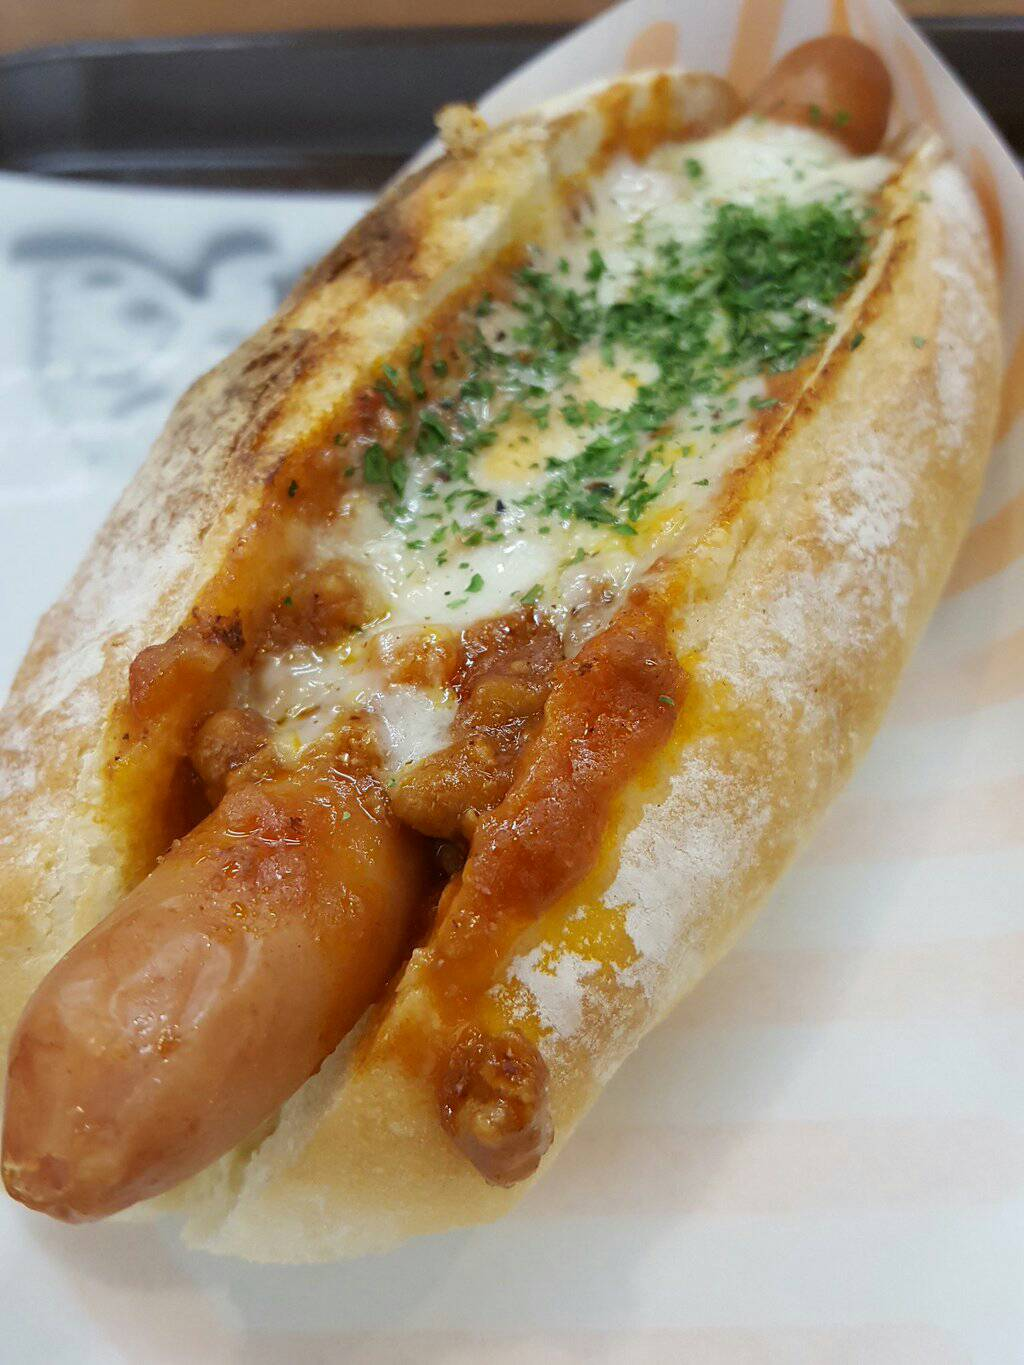
\includegraphics[width=6cm]{image1}
  \caption{入力画像}
\end{figure}
今回はこの画像を使用する。
\begin{figure}[H]
  \centering
  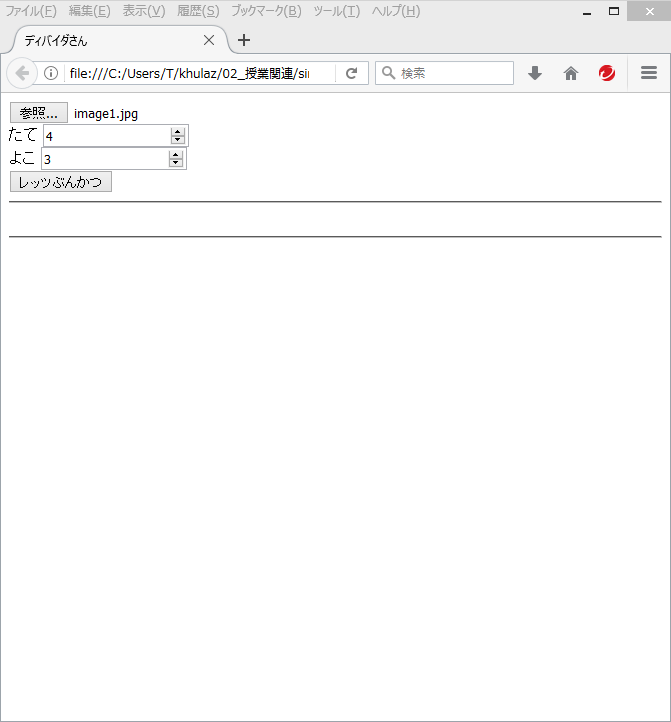
\includegraphics[width=6cm]{pr1}
  \caption{起動直後}
\end{figure}
photo\_divider.htmlを開くとブラウザ上に上記のようなページが表示される。
\begin{figure}[H]
  \centering
  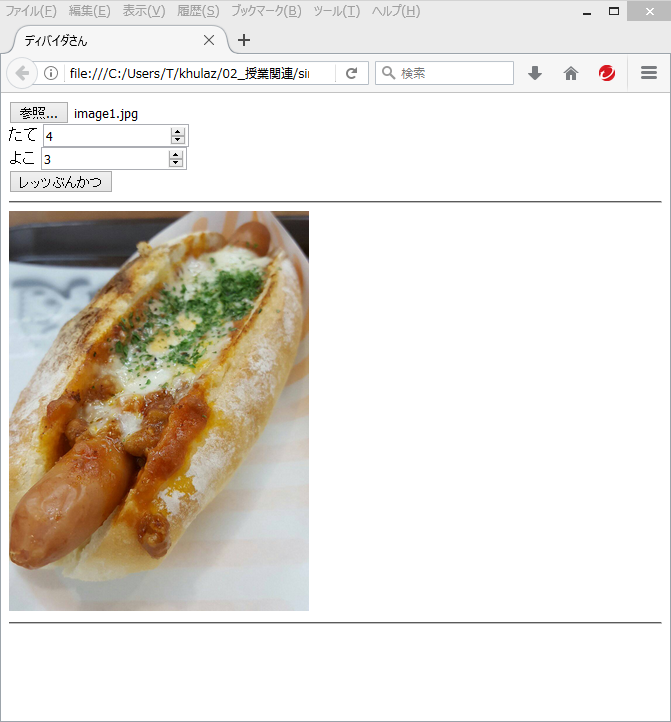
\includegraphics[width=6cm]{pr2}
  \caption{画像選択後}
\end{figure}
画像を選択後、数値を入力して分割数を決定する。
\begin{figure}[H]
  \centering
  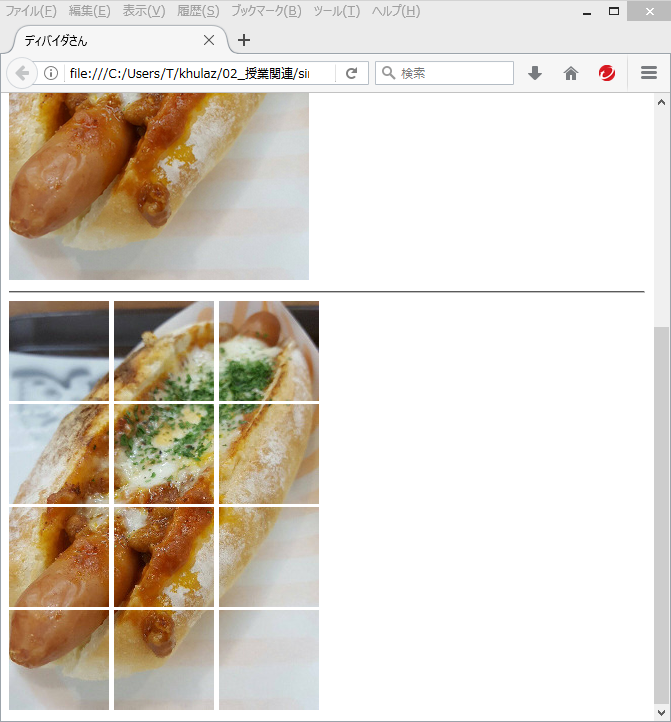
\includegraphics[width=6cm]{pr3}
  \caption{分割処理後}
\end{figure}
確かに、画像が指定数分割されていることが分かる。
\section{プログラム操作説明}
\begin{enumerate}
 \item 分割したい画像を参照ボタンから選択します。
 \item 縦、横の分割数を入力します。(1~64の範囲内で指定してください。)
 \item ”レッツぶんかつ”ボタンを選択すると分割された画像がページ下部に表示されます。
\end{enumerate}
※分割数を大きくし過ぎた場合ブラウザの動作が遅くなる場合があります。\\
※分割を再度行いたい場合は一度ページを更新して再度①の手順から行ってください。\\

\section{プログラム仕様説明}
入力画像のファイル形式はbmp,png,jpgとする。出力画像のファイル形式はjpgとなる。
出力された画像は、一行に横の分割数分、縦の分割数の行数分だけ出力される。例えば、縦を3、横を4と指定した場合「一行あたり4枚の画像が3行分、合計12枚の画像」が出力される。\\
プログラムは、アプリケーションの本体であるphoto\_divider.htmlと、アプリケーションの動作を記述したdivider.jsから成る。HTML内のボタンがdivider.jsに実装されたメソッドを呼び出し、画像の分割を行う。
divider.jsのDivideメソッドが画像の分割作業の本体を担う。このメソッドは、入力画像と分割数をHTMLのタグから取得し、分割数に応じてHTMLにimageタグを追加し、そこに元画像を分割した画像ファイルを生成して書き込んでいく。

\section{考察}
画像の分割にかかる時間は横の分割数をn、縦の分割数をmとするとO(nm)になると考えられる。

\section{所感}
javascriptとHTML5を利用したDLやインストールといった手順を必要としないアプリケーションやサービスはユーザーが利用するための敷居を大きく下げることに一役買ってくれるはずなので、今後も追求していきたい。

\section{参考URL}
\noindent
javascriptで画像処理してみよう(1)〜OpenCVjs〜\\
\noindent
”http://ameblo.jp/sakiyamak/entry-11382031239.html”

\end{document}